\documentclass[a4paper, 11pt]{article}

\usepackage[margin=1in]{geometry}

\usepackage{hyperref}
\usepackage{graphicx}
\usepackage{graphics}
\usepackage{verbatim}
\usepackage{listings}
\usepackage{color}

\begin{document}

\title{The BANO protocol design and implementation}
\author{BANO team}
\date{}

\maketitle

%% \newpage
%% \tableofcontents
%% \addtocontents{toc}{\protect\setcounter{tocdepth}{1}}


\clearpage
\section{BANO protocol design}

\subsection{Overview}
\paragraph{}
The BANO protocol has been designed to implement a wireless network where a
resourceful device known as the base interacts with smaller devices known as
the nodes. The protocol especially targets domotics applications, but is not
limited to them.

\paragraph{}
In a typical architecture, the base centralizes node information. The base
reports node information to the user, and schedules appropriate actions based
on the user configuration.

\paragraph{}
To ease conceptual understanding, this document focuses on the common case where
base and node roles are clearly distinct. However, there is no limitation that
prevents a node to act as a base, and a base to act as a node. Also, the protocol
does not limit the base count.

\paragraph{}
The BANO protocol is used between bases and nodes for accessing key value pairs
using 2 basic operations:
\begin{itemize}
\item the \textit{SET} operation is used to set a value given a specific key,
\item the \textit{GET} operation is used to get a value given a specific key.
\end{itemize}

\begin{figure}[!h]
\begin{center}
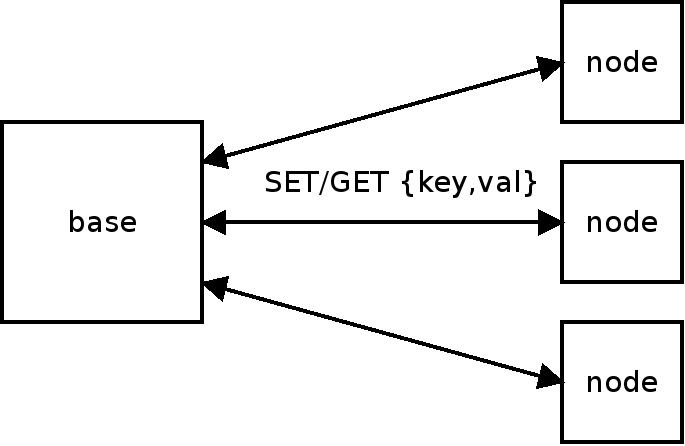
\includegraphics[scale=0.2]{../dia/overview_keyval/main.jpeg}
\end{center}
\caption{\tiny{key value exchange}}
\label{overview_keyval}
\end{figure}

\paragraph{}
These 2 operations are used to implement the following:
\begin{itemize}
\item \textit{synchronous SET} with optionnal acknowledgement: a base can set a
node value by sending a \textit{SET} message. If required, an acknowledgement can
be sent back as a flagged message,
\item \textit{synchronous GET}: a base can get a node value by sending a
\textit{GET} message, and wait for the corresponding reply,
\item \textit{asynchronous SET}: a base can get a node value by listening for
\textit{SET} messages coming from nodes.
\end{itemize}


\subsection{Design considerations}

\subsubsection{Focus on common case}
\paragraph{}
The protocol is designed with common case in mind. Any feature that is not
mandatory should not impact its design. For instance, security is a feature
that would impact message format if made mandatory. Another example is the
lack of message routing support.

\subsubsection{Node simplicity}
\paragraph{}
Nodes resource requirements should be as low as possible, enabling low cost
8 bits microcontroller based configurations. On the contrary, the base is
considered resourceful. This should be used to lower the node requirements.

\subsubsection{Low power consumption}
\paragraph{}
\textbf{TODO}
%% TODO: node mode (passive, listen only, time ...)

\subsubsection{Low memory footprint}
\paragraph{}
\textbf{TODO}


\subsection{Transport layer}
\paragraph{}
BANO aims at being independent from the physical layer and limits the
constraints put on the layer used to transport messages. It requires:
\begin{itemize}
\item packet ordering is not required,
\item packet acknowledgement is not required,
\item a fixed size packet based transport layer,
\item if provided by hardware, addressing must be at least 4 bytes.
Otherwise, addressing is implement in software and the payload size must be
increased by 4 bytes,
\item if implemented by hardware, the CRC must be at least 2 bytes. Otherwise,
the CRC can be implemented in software,
\item data payload size must be at least 16 bytes, and depends on what is
implemented in software.
\end{itemize}

\paragraph{}
The physical layer can work in all the commonly used wireless ranges (433, 868,
915 MHz and 2.4 GHz). 2 chipsets are considered:
\begin{itemize}
\item NRF905
\item NRF24L01P
\end{itemize}


\subsection{Addressing}
\paragraph{}
Network nodes are addressed using 32 bits identifiers. Addresses are randomly
generated at programming time, along with a random 32 bits seed. At any time,
the base can detect address collision by checking the uniqueness of the
addr,seed pair. To do so, it sends a message to all the nodes that it has
currently discovered:
%% msg.daddr = node_addr
%% msg.hdr.op = BANO_OP_GET
%% msg.hdr.flags = 0
%% msg.hdr.saddr = base_addr
%% msg.u.set.key = BANO_KEY_ADDR

\paragraph{}
Nodes reply with the following message:
%% msg.daddr = base_addr
%% msg.hdr.op = BANO_OP_SET
%% msg.hdr.flags = BANO_FLAG_REPLY
%% msg.hdr.saddr = node_addr
%% msg.u.set.key = BANO_KEY_ADDR
%% msg.u.set.val = node_seed

\paragraph{}
If there are 2 random ids for one address, a collision is detected. The base
resolves the conflict and sends new addresses to the node:
%% msg.daddr = node_previous_addr
%% msg.hdr.op = BANO_OP_SET
%% msg.hdr.flags = 0
%% msg.hdr.saddr = node_new_addr
%% msg.u.set.key = BANO_KEY_ADDR
%% msg.u.set.val = node_seed

\paragraph{}
%% By default, the base uses the BANO_DEFAULT_BASE_ADDR address.


\subsection{Messaging}
\paragraph{}
%% in RX mode, a node receive logic consumes power. to reduce power consumption and
%% avoid being, a node can poll the requests by sending a request:
%% BANO_OP_GET, BANO_KEY_REQ, node_addr
%% the base must then send requests for this node in a short time lapse, and the
%% node will then return to reduced power mode at completion.
%% also, note the polling scheme prevents a malicious sender to
%% keep transmitting to a node in order to reduce its battery life.

%% TODO
%% [ on message forwarding ]
%% Some physical setup may require the use of repeater.

\paragraph{}
TODO: message integrity

\paragraph{}
TODO: message acknowledgement


\subsection{Security}
\paragraph{}
%% Implementing security adds complexity not required in all cases and goes against
%% some other BANO protocol design choices (stateless, common case, short message
%% size). However, it is undeniable that there are node messages that require some
%% or all of the following security features:
%% . hiding message contents
%% . preventing replay attack
%% . preventing brute force
%% . preventing tampering attacks (mim ...)
%% . detecting flood
%% . node DOS


%% [[ message contents hiding ]]

%% Symetric block ciphers can be used to hide message contents. The cipher
%% block size should comply with the BANO message size, ie. 16 bytes. Thus,
%% a 128 bits cipher is chosen (AES 128). Also, encryption is enabled for
%% all the messages of a given node. If this is a limitation, a node key
%% can allow the node to switch switch the encryption mode. In this case,
%% and because of statelessness, the encryption mode toggling should be
%% sent in 2 encrypted and clear versions.

%% Ciphers rely on a secret key shared between the base and the node. There
%% is no support for sharing the key built in the protocol. In a typical
%% situation, the node is programmed with a random key that is made known
%% to the base using the configuration interface.


%% [[ preventing replay attack ]]

%% The usual way to prevent replay attack is for the node message to convey
%% a seed. This seed must not be known by the attacker at the time the message
%% is generated.

%% example: shutting down an alarm
%% An attacker may replay a previously capture message used to
%% unlock an alarm, even if encrypted. If the message contains
%% a time dependent information that can be checked by the base,
%% then any previously generated message will no longer be valid.
%% The time dependent information should be generated randomly
%% in a fashion not known by the attacker. For instance, a seed
%% can be generated locally by the base and sent encrypted to
%% the node.

%% [[ preventing brute force ]]

%% [[ preventing tampering attacks (mim ...) ]]

%% a hash of the message payload is included in the message. the message
%% is then encrypted. Thus, a modification


%% [[ detecting node flood ]]
%% flood can be used or to prevent a node from speaking with
%% the base.


%% . security seed broadcast
%% -> the master (node?) broadcasts a seed at regular interval his security
%% seed is used in the encryption token scheme
%% -> if the node broadcast, it must be able to generate it, which means random
%% number generation caps
%% -> if the master broadcast it, the node has to store it

%% => any failed attempt to check the security token should renegotiate the
%% node security context

%% TODO
%% [ on the assumption base is always present before nodes ]

%% A scenario where the user powers a node before powering the
%% base is largely possible. Handshaking .

%% Also, the base could be powered

%% Also, completely passive nodes (ie. alarm) does not anounce
%% themselves when powered up.

%% Thus, the base is not assumed to be present when a node is
%% added to the network.

%% (or base cannot assume base was present at the time
%% they do). Thus, there must be a mechanism to convey every
%% required information in one message.

%% Designing the protocol this way will increase



\section{BANO protocol implementation}

\subsection{Message format}

\paragraph{}
A message consists of a 128 bits sequence (16 bytes). Any field wider than 1
byte uses the little endian encoding. A header is always present and its format
is common to all the messages. The payload varies according to the operation
field.

\paragraph{}
\begin{figure}[!h]
\begin{center}
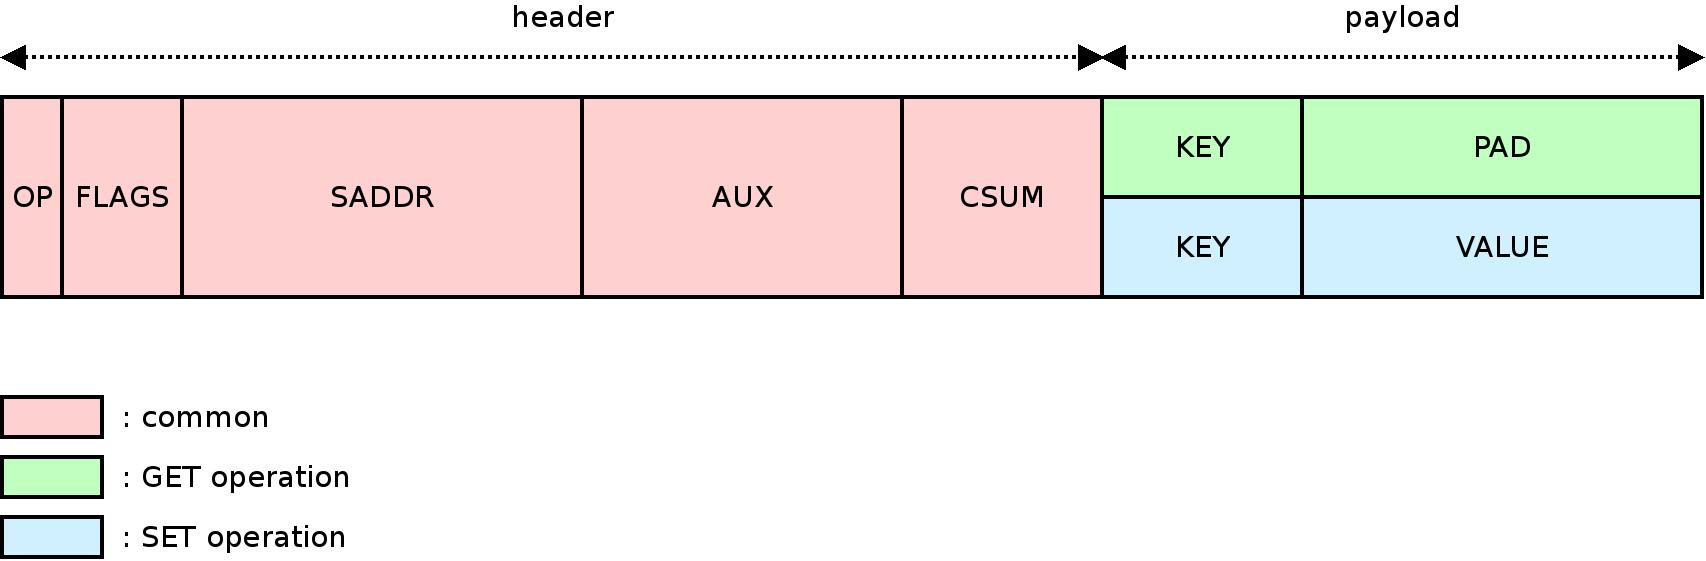
\includegraphics[scale=0.2]{../dia/implem_format/main.jpeg}
\end{center}
\caption{\tiny{message format}}
\label{implem_format}
\end{figure}


\paragraph{}
The following section details the message fields.

\subsubsection{OP, 2 bits}
\paragraph{}

\subsubsection{FLAGS, 6 bits}
\paragraph{}

\subsubsection{SADDR, 32 bits}
\paragraph{}

\subsubsection{AUX, 24 bits}
\paragraph{}

\subsubsection{CSUM, 16 bits}
\paragraph{}

\subsubsection{KEY, 16 bits}
\paragraph{}
%% \textit{keys} are 16 bits identifiers. Each node exposes a set of predefined
%% keys and a set of specific keys.

\subsubsection{VALUE, 32 bits}
\paragraph{}
%% \textit{value} are 32 bits wide. The protocol does not specify a format for
%% this field. For instance, it can be used to transmit integer or real values.
%% The base uses the node description file to interpret the value of a specific
%% key.


\subsubsection{PAD, 32 bits}
\paragraph{}


\end{document}
